% !TEX program = pdflatex
% Draft extracted from the repository evidence at tag v0.1.0.
% Every number in this file traces to a tracked artifact under results/ or to
% NOTES.md; do not edit a number here without editing its source first.
%
% CITATION DISCIPLINE (repo rule: read before citing):
%   - Verified by direct fetch during the 2026-08-06 review rounds:
%       arXiv 2606.22916 (IGAC), 2607.05397 (Proof of Execution).
%   - Audited in the repository's 2026-08-06 citation round:
%       arXiv 2606.09863 (Advani), 2603.03116 (Cao), 2512.07850 (SABER),
%       2604.07911 (DACS), MCP tool-annotations posts.
%   - Verified by direct fetch, 2026-08-06 (resolves the former pending
%       entry): arXiv 2607.08028 (Ahn & Kim, harness engineering) --
%       cited with delimitation in Related work.
%   - Verified against the downloaded 1983 PDF (pp. 289-290), 2026-08-06:
%       Haerder & Reuter, "Principles of Transaction-Oriented Database
%       Recovery" -- both quoted sentences ("commits only legal results";
%       "can only be removed by countertransactions") are verbatim. Note:
%       the source says "legal results", NOT "declared integrity
%       constraints" -- the paper deliberately quotes their terms.
%   - Verified against the downloaded HotOS 2017 PDF, 2026-08-06:
%       Huang et al., "Gray Failure" -- the quoted definition ("when at
%       least one app makes the observation that system is unhealthy, but
%       observer observes that system is healthy") is verbatim from S3.2;
%       observer/reactor part of the system, app external (S3.1); author
%       list verified from the paper's first page.
%   - Verified by direct fetch of the FULL TEXT, 2026-08-06: arXiv
%       2606.14589 (Wei Wu, silent-failure taxonomy) -- the body uses
%       gray-failure / differential-observability vocabulary, cites
%       Huang et al. 2017 as its reference [1], and class C ("error
%       swallowing and dilution") covers absorption of malformed
%       responses into downstream fields. Citation upgraded accordingly.

\documentclass[11pt]{article}

\usepackage[a4paper,margin=1in]{geometry}
\usepackage[T1]{fontenc}
\usepackage[utf8]{inputenc}
\usepackage{booktabs}
\usepackage{array}
\usepackage{microtype}
\usepackage{xcolor}
\usepackage{colortbl}
\usepackage{tikz}
\usetikzlibrary{arrows.meta,positioning,calc}
\usepackage[hidelinks]{hyperref}

\newcommand{\cellA}{\textsf{A}}
\newcommand{\cellB}{\textsf{B}}
\newcommand{\cellC}{\textsf{C}}
\newcommand{\cellD}{\textsf{D}}
\newcommand{\statuscompleted}{\texttt{completed}}
\newcommand{\statusfailedclean}{\texttt{failed\_clean}}

\title{Telemetry Blindness at the Agent--Business Boundary:\\
A Controlled Measurement of Output-Contract Enforcement}

\author{Estefano Senhor Ferreira\\
\small\texttt{estefano.senhor@gmail.com}}

\date{Draft --- extracted from repository state \texttt{v0.1.0}, 2026-08-06}

\begin{document}
\maketitle

\begin{abstract}
LLM agents that write business state can report success while persisting
corrupted records. We reproduce this failure as a controlled six-cell
comparison (plus a control arm) --- \emph{decoding constraint}
(provider-enforced response schema vs.\ schema stripped) crossed with
\emph{boundary policy} (tolerant repair vs.\ a strict
retry-once-then-fail output-contract guard), a fault injector forcing
format violations in the unconstrained cells and, in two pre-registered
follow-up cells, downstream of the active schema --- on one codebase and
one model, with ground truth read directly from the persisted SQLite of
an external system of record. Two findings
carry the paper. First, \emph{telemetry blindness}: with repair
positioned before the contract check, the tolerant configuration
reported success 10/10 and persisted ten garbage business records while
every platform-side instrument --- status, contract counters, repair
count --- read success or no violation; only the database showed the
corruption. The signature reproduced unchanged with the schema active
and the fault injected downstream of it --- a pre-registered follow-up
whose opposite prediction (that fence-stripping repair would recover the
valid content under the fence) the data falsified. Second, the guard's
price sheet: under enforced decoding
both boundary policies were byte-equivalent and the guard's idle cost
was zero (natural violations 0/10 --- a bounded observation, not an
elimination claim); when a violation does arrive, the strict guard's
price is one extra model call, buying typed, unpersisted failure instead
of silent corruption --- a trade a naturally occurring provider
schema-dialect mismatch exercised for us. The implication is
deliberately narrow: constrained decoding is the suppression mechanism;
the architectural boundary is what keeps the channel closed when that
simpler mechanism silently breaks. All evidence is version-controlled
and inspectable.
\end{abstract}

\section{Introduction}

The failure this paper measures was first observed in the wild, not
designed. Ten consecutive executions of an email-to-ERP business flow
reported success; ten times, the ERP received a truncated, markdown-fenced
JSON blob as the customer-facing \texttt{summary} field --
indistinguishable from a legitimate record to any downstream consumer. The
platform's contract counters read zero violations: a tolerant parser
``repaired'' each response before any check could see it. Every
authorization held. The business API's own validation passed --- the
corruption was in \emph{content}, and content of valid form.

The gap has a name older than agents. Transaction processing drew this
line four decades ago: in the paper that coined ACID, a committed
transaction ``by definition commits only legal results'' --- and, in the
same discussion, ``since, by definition, each transaction is correct,
the effects of an inevitable incorrect transaction (i.e., the
transaction containing faulty data) can only be removed by
countertransactions''~\cite{haerder1983}. Consistency guarantees
legality by the database's lights; correctness of the written content is
\emph{assumed}, not guaranteed. What has changed is the writer, not the
guarantee. Under programmatic writes the gap is rarely exercised: code
writes what the programmer specified, so a semantically wrong value of
valid form is the exception. Under LLM generation, form is enforced at
the decoder while content is probabilistic --- the gap goes from rarely
exercised to routinely exercised. That is why business validity, which
could remain an implicit programmer responsibility, needs an explicit
owner when the content author is stochastic.

The phenomenon is not idiosyncratic. Advani measures \emph{false success}
--- an agent claiming completion with no corresponding state change in the
system of record --- at 45--48\% of failures in single-control
\mbox{$\tau^2$-bench} domains, and finds LLM judges fail to detect it
(AUROC $\le 0.65$)~\cite{advani2026}. Cao et al.\ find 27--78\% of
benchmark-reported successes to be procedurally corrupt~\cite{cao2026}.
SABER localizes the damage: deviations in \emph{mutating} steps reduce
task-success odds by up to 92--96\%, while deviations in non-mutating
steps have little effect~\cite{saber2025} --- the write path is where
failures become decisive.

What the literature does not settle is an engineering question.
Provider-enforced structured output (constrained decoding) now exists and
demonstrably works --- so the question that can actually be answered with
measurements is conditional: \emph{when decoding enforcement silently
fails, what does each boundary policy between generated content and the
business write do with the violation --- and what does keeping the
stricter policy cost while decoding still works?} This paper answers
with a controlled measurement
whose ground truth is not the agent's report, not the platform's
telemetry, but rows in the business database.

\paragraph{Contributions.}
(1)~A controlled comparison of four boundary configurations --- decoding
enforcement crossed with boundary repair policy, a fault injector in the
unconstrained column, and a shared control arm --- with ground truth read
from a persisted external system of record. The design is not a complete
factorial (\S\ref{sec:design}); what this measurement adds is the
database-grounded reading: outcomes judged against rows in the business
store rather than against agent reports or platform telemetry.
(2)~The measured finding that \emph{tolerant repair conceals rather than
repairs}, and specifically that it blinds the platform's own integrity
counters --- the audit trail records zero violations in the cell that
persists 100\% garbage: the \emph{telemetry blindness} defined in
\S\ref{sec:results}.
(3)~An honest pricing of the boundary guard as insurance: idle cost zero
when decoding enforcement works, one extra model call per violation when
it does not, and a naturally occurring configuration failure in which the
insurance paid out.

\section{The measured system}
\label{sec:system}

The reference implementation is a minimal agent platform for business
process automation (three agents, eight tools, two human-authored plans)
in which non-determinism is confined to three model decisions: plan
selection, capability selection, and content generation. Step order is
declared in versioned YAML; the model never decides what runs next. Three
properties matter for this experiment:

\begin{enumerate}
\item \textbf{External system of record.} Business writes go through an
ERP service (SQLAlchemy over SQLite) that owns its invariants as database
constraints and rejects violations with typed errors. The platform holds
no business entity. Ground truth for every cell is read from this
database, never from platform state.
\item \textbf{Output contract on the write path.} The \emph{boundary} is
the single interface through which generated content becomes business
state. Generated content that
feeds a business write is validated against a declared schema at a
boundary the generator cannot bypass; on violation, at most one retry,
then a typed failure --- nothing unvalidated persists. This is the
mechanism under test.
\item \textbf{Unsampled audit.} Proposals, policy decisions, business
validations, output-contract events and compensations are recorded
append-only, as distinct kinds. The experiment measures, among other
things, whether this trail can be trusted --- it cannot, in one cell, for
a reason worth stating precisely (\S\ref{sec:results}).
\end{enumerate}

The pattern's full specification and its seven load-, registration- and
runtime-enforced restrictions are in the repository; none of them is the
subject here. The subject is the boundary between generated content and
persisted business truth.

\section{Experimental design}
\label{sec:design}

\paragraph{Axes.} \emph{Decoding constraint}: the provider-enforced JSON
schema (\texttt{responseSchema}) either passed through to the model
provider, or stripped by an infrastructure decorator
(\texttt{SchemaStrippingClient}). \emph{Boundary policy}: either a strict
output-contract guard (\texttt{retry\_once\_then\_fail}) or a tolerant
repair decorator (\texttt{TolerantRepairClient}) that strips markdown
fences well enough to satisfy the parser and passes the result through ---
an emulation, as an infrastructure decorator, of the historical fallback
behavior that produced the original incident. Construct validity requires
one precision: the historical fallback lived \emph{inside the
capability's parser} (after a parse failure it stuffed the fenced blob
into the business field); the emulation reconstructs that behavior as an
infrastructure decorator so that measurement never touches the platform's
behavior layer. The comparison is therefore against a reconstruction at a
different layer --- and what transfers is positional, not layer-specific:
any absorption upstream of the contract check blinds the counters the
same way (Figure~\ref{fig:order}).

\paragraph{Fault injection.} Cells \cellA{} and \cellB{} (no schema)
additionally run a generation-fault injector
(\texttt{GenerationFaultInjectionClient}) that re-fences \emph{every}
generation response. The violation rate in these cells is therefore forced
by construction --- 10/10 measures the injector, not the model. This is
deliberate: the natural no-schema violation rate on this model was
measured in an earlier round (10/10 fenced --- itself an artifact of
flash-tier defaults under prompt-only control), and the question this
matrix asks is conditional: \emph{given} a violation, what does each
configuration do with it? The injector also re-fences the retry attempt,
so recovery in cell \cellB{} is impossible by construction; the guard's
failure path, not its recovery path, is what \cellB{} measures.

Stated plainly: because the injector runs only in the no-schema cells,
\textbf{the design is not a complete factorial} --- the fault arm
co-varies with the decoding axis. Cells \cellC{}/\cellD{} measure the
schema configuration under \emph{natural} conditions only; no cell in
this matrix subjects active decoding enforcement to a forced violation.
The findings are worded accordingly (F3 claims invisibility of the
repair axis and zero idle cost, not that decoding ``holds under
attack''), and the missing cells are discussed in \S\ref{sec:limits}.

\paragraph{Cells and control.} Ten repetitions per cell of the two-agent
email-to-ERP plan (the only plan with a generation step), each against a
fresh SQLite file. A control arm runs the \cellD{} configuration on the
no-generation scheduling plan (3 repetitions): the axes should touch
nothing but the generation step. Model: \texttt{gemini-3.1-flash-lite},
same prompts throughout; everything varies by command-line flags only.

\paragraph{What is read as the result.} Reported status; contract
violation/retry/failure counters from the audit trail; repair count; rows
created in the ERP database; per-row validity of the persisted
\texttt{summary} (checked by direct SQL inspection, not via any platform
report); tokens and cost.

\paragraph{Price basis.} Cost figures are computed by the runner from the
per-model pricing table in the platform's observability writer:
for \texttt{gemini-3.1-flash-lite}, \$0.25 per million input tokens and
\$1.50 per million output tokens, rates as recorded on 2026-07-28 from
the official pricing page
(\url{https://ai.google.dev/gemini-api/docs/pricing}). Token counts come
from the provider's own \texttt{usage\_metadata}
(\texttt{prompt\_token\_count}, \texttt{candidates\_token\_count} plus
thought tokens where the model reports them,
\texttt{cached\_content\_token\_count}), not from an estimator. Cached
input is billed at 10\% of the input rate in the runner's formula; in
these runs cached tokens were zero --- verified by recomputing all 43
recorded per-execution costs from their token counts alone, which
reproduces every recorded figure exactly
(\texttt{scripts/verify\_costs.py} in the repository). All runs executed inside
free-tier quota, so the figures are list-price equivalents, not amounts
billed. List prices change; the figures are reproducible against the
rates as of the stated date, and the token counts --- which do not change
--- are in the tracked evidence files
(\texttt{results/integrity-matrix/integrity\_matrix.jsonl}, per
(cell,~rep)).

\section{Results}
\label{sec:results}

\begin{table}[t]
\centering
\small
\begin{tabular}{@{}lllrrrrr@{}}
\toprule
Cell & Configuration & Status (10 reps) & Viol./Retry/Fail & Repairs &
Rows & Valid & Cost \\
\midrule
\cellA{} & no schema + fault + tolerant & \statuscompleted{} 10/10 & 0/0/0
& 10 & 10 & \textbf{0} & \$0.00304 \\
\cellB{} & no schema + fault + strict & \statusfailedclean{} 10/10 &
10/10/10 & 0 & \textbf{0} & --- & \$0.00509 \\
\cellC{} & schema + tolerant & \statuscompleted{} 10/10 & 0/0/0 & 0 & 10 &
10 & \$0.00247 \\
\cellD{} & schema + strict & \statuscompleted{} 10/10 & 0/0/0 & 0 & 10 &
10 & \$0.00246 \\
ctrl & \cellD{} config, no-generation plan & \statuscompleted{} 3/3 &
0/0/0 & 0 & 3 & n/a & \$0.00017 \\
\midrule
E & schema + fault + tolerant & \statuscompleted{} 10/10 & 0/0/0
& 10 & 10 & \textbf{0} & \$0.00245 \\
F & schema + fault + strict & \statusfailedclean{} 10/10 &
10/10/10 & 0 & \textbf{0} & --- & \$0.00384 \\
\bottomrule
\end{tabular}
\caption{The integrity matrix. ``Rows'' are records created in the
external ERP database; ``Valid'' counts rows whose persisted
\texttt{summary} is clean one-line text (verified by direct SQL
inspection). Cell \cellA{}'s ten rows each carry a double-fenced JSON blob
in the business field while every counter the platform exposes reads
zero. Below the rule: the pre-registered follow-up cells E and F
(\S\ref{sec:limits}), run after the original comparison --- E reproduces
\cellA{}'s signature with the decoding constraint active upstream.
Latency means are omitted: they are contaminated by free-tier
429-backoff stalls (worst case 111\,s) and carry no signal about the
axes.}
\label{tab:matrix}
\end{table}

\paragraph{F1 --- without the schema, the boundary alone separates the
outcomes.} Same fault, same model, same pipeline: \cellA{} reports
\statuscompleted{} 10/10 and persists 10 garbage business records;
\cellB{} reports \statusfailedclean{} 10/10 and persists zero. One
epistemic asymmetry must be stated: \cellB{}'s outcome is deterministic
by construction (the injector re-fences the retry and the guard is coded
to fail typed), so \cellB{} \emph{verifies}, under real-model conditions,
that the strict policy does what its code says --- a designed contrast,
not a discovery. The discovery is in \cellA{}, and it is emergent rather
than programmed: the corrupted content does not merely evade the check
--- it reaches the business database while every platform-side
instrument reads clean (F2).

\paragraph{F2 --- tolerant repair conceals, and blinds the telemetry.}
Cell \cellA{}'s contract counters read 0/0/0 because the repair runs
\emph{before} the contract check ever sees the response; only the repair
count (10) and direct database inspection reveal what happened. The
practitioner literature warns in prose that syntactic repair ``fixes
syntax, not semantics''; part of it celebrates high repair-success rates
as a virtue. The matrix quantifies the inverted reading: ``repaired''
10/10, valid 0/10. The consequence extends a lesson the false-success
literature draws about agent self-reports~\cite{advani2026,cao2026} one
level deeper: in a repair-before-check pipeline, \emph{the platform's own
integrity telemetry is not evidence either}. Only the system of record is
(Figure~\ref{fig:observers}); and the mechanism is positional, not a
property of repair itself (Figure~\ref{fig:order}). Two levels of this
claim must be kept apart. The \emph{positional} mechanism is general:
any absorption upstream of a check blinds the counters that check feeds.
The \emph{measured} result is narrower: format repair ahead of a format
check. A repair that normalizes content ahead of a form check, or form
repair ahead of a semantic check, was not tested and may behave
differently (\S\ref{sec:limits}).

\begin{figure}[t]
\centering
\small
\begin{tabular}{@{}lccc@{}}
\toprule
 & Cell \cellA{} & Cell \cellB{} & Cell E \\
 & (no schema, tolerant) & (no schema, strict) & (schema, tolerant) \\
\midrule
\rowcolor{gray!12}
\multicolumn{4}{@{}l@{}}{\itshape what the platform reports} \\
Agent report & \statuscompleted{} 10/10 & \statusfailedclean{} 10/10 &
\statuscompleted{} 10/10 \\
Contract counters (viol.\,/\,retry\,/\,fail) & 0 / 0 / 0 & 10 / 10 / 10 &
0 / 0 / 0 \\
Repair count & 10 & 0 & 10 \\
\midrule
\rowcolor{gray!12}
\multicolumn{4}{@{}l@{}}{\itshape what the database holds} \\
Rows in ERP & 10 & 0 & 10 \\
Valid rows & \cellcolor{gray!25}\textbf{0} & --- &
\cellcolor{gray!25}\textbf{0} \\
\bottomrule
\end{tabular}
\caption{What each observer sees (data from Table~\ref{tab:matrix}; no
new measurement). The separation between the two bands is the finding:
in cells \cellA{} and E, three platform-side instruments agree the runs
succeeded --- status \statuscompleted{}, contract counters at zero, ten
``successful'' repairs --- while the business database holds ten
corrupted records and zero valid ones. Cells \cellA{} and E differ in
decoding condition (schema stripped vs.\ active, the fault injected
downstream of it): the same blindness signature in both columns is
Proposition~1's positional claim (\S\ref{sec:results}), visible at a
glance.}
\label{fig:observers}
\end{figure}

\begin{figure}[t]
\centering
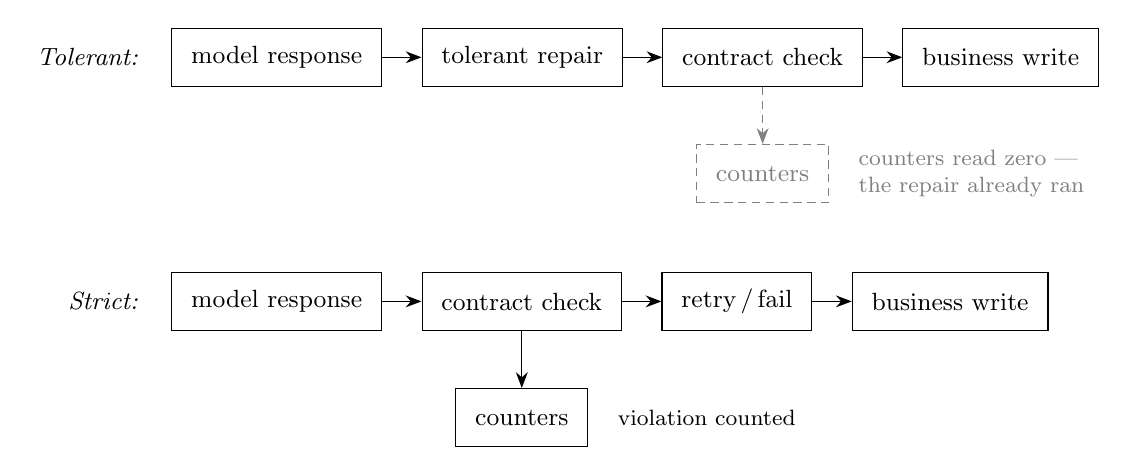
\begin{tikzpicture}[
  stage/.style={draw, rectangle, minimum height=2.1em, inner xsep=7pt,
                font=\small},
  rowlbl/.style={font=\small\itshape, anchor=east},
  note/.style={font=\footnotesize, align=left},
  >={Stealth[length=2mm]}]
% tolerant pipeline
\node[rowlbl] (tl) at (0,0) {Tolerant:};
\node[stage, anchor=west] (t1) at (0.3,0) {model response};
\node[stage, anchor=west] (t2) at ($(t1.east)+(0.5,0)$) {tolerant repair};
\node[stage, anchor=west] (t3) at ($(t2.east)+(0.5,0)$) {contract check};
\node[stage, anchor=west] (t4) at ($(t3.east)+(0.5,0)$) {business write};
\draw[->] (t1) -- (t2);
\draw[->] (t2) -- (t3);
\draw[->] (t3) -- (t4);
\node[stage, densely dashed, draw=gray, text=gray]
  (tc) at ($(t3.south)+(0,-1.1)$) {counters};
\draw[->, densely dashed, gray] (t3) -- (tc);
\node[note, text=gray, anchor=west] at ($(tc.east)+(0.25,0)$)
  {counters read zero ---\\ the repair already ran};
% strict pipeline
\node[rowlbl] (sl) at (0,-3.1) {Strict:};
\node[stage, anchor=west] (s1) at (0.3,-3.1) {model response};
\node[stage, anchor=west] (s2) at ($(s1.east)+(0.5,0)$) {contract check};
\node[stage, anchor=west] (s3) at ($(s2.east)+(0.5,0)$) {retry\,/\,fail};
\node[stage, anchor=west] (s4) at ($(s3.east)+(0.5,0)$) {business write};
\draw[->] (s1) -- (s2);
\draw[->] (s2) -- (s3);
\draw[->] (s3) -- (s4);
\node[stage] (sc) at ($(s2.south)+(0,-1.1)$) {counters};
\draw[->] (s2) -- (sc);
\node[note, anchor=west] at ($(sc.east)+(0.25,0)$) {violation counted};
\end{tikzpicture}
\caption{Why F2 happens: one position in the sequence, not a property of
repair. In the tolerant pipeline the repair runs before the contract
check, so the check --- and the counters it feeds --- never see the
violation; in the strict pipeline the check runs first and the violation
is counted before retry or typed failure.}
\label{fig:order}
\end{figure}

\paragraph{Definition 1 (Telemetry blindness).} A pipeline exhibits
\emph{telemetry blindness} when every platform-side observer reports
success or no violation while the system of record holds corrupted
state.

\paragraph{Proposition 1 (Sufficient condition).} Given a violation
that reaches persistence, any absorption step positioned upstream of
the check that feeds those observers suffices: the check never sees the
violation, so the counters it feeds cannot record it --- and the
absorption step's own counter reads as successes, not violations. The
condition is mechanism-agnostic: it holds for any absorption step, not
only the format repair measured here (the measured narrowing above
stands).

\paragraph{Observed instance.} Cell \cellA{}: agent report
\statuscompleted{}, contract counters at zero, repair count reporting
ten successes, ten corrupted rows in the business database. A second
instance was measured after this definition was written and
pre-registered (\S\ref{sec:limits}): the same signature --- counters at
zero, ten repairs, ten corrupted rows --- with decoding enforcement
active upstream and the fault injected downstream of it. The condition
is positional, indifferent to what sits upstream of the absorption.

\paragraph{F3 --- with the schema, no violation occurred and the repair
axis is invisible.} Cells \cellC{} and \cellD{} are byte-equivalent in
outcome (10 clean rows each, $\sim$same tokens, $\sim$same cost) with
zero natural violations at $N{=}10$ --- an observation bounded at
$\le 25.9\%$ (\S\ref{sec:limits}), not an elimination claim, and these
cells never faced a forced violation (\S\ref{sec:design}). The direct
evidence that decoding-level enforcement suppresses \emph{natural}
violations is the earlier before/after round on the same pipeline: 10/10
violations under prompt-only control $\rightarrow$ 0/10 with the schema,
at $-18\%$ cost per completed task. What \cellC{}/\cellD{} add is the
guard's price sheet: under the enforced-decoding configuration the guard
has literally nothing to do, and its idle cost --- extra model calls,
extra tokens --- is zero.

\paragraph{F4 --- the guard's price is one extra call per violation.}
\cellB{} spent $\sim$2$\times$ \cellA{}'s output tokens (\$0.00509 vs.\
\$0.00304 per 10 reps): the retry doubles the generation call and both
attempts fault by construction. That is the entire price of knowing.

\paragraph{F5 --- the control arm isolates the generation step.} The
no-generation plan completed 3/3 with clean persisted state under the
\cellD{} configuration: the axes touch nothing else in the pipeline.

\section{The naturally occurring case}
\label{sec:accident}

The matrix's guarded no-schema cell models a configuration class that
occurred naturally during the study, unplanned. The first corrected
measurement round passed the output schema through the provider's
\texttt{response\_schema} config field --- which accepts an OpenAPI-subset
dialect and rejected the standard JSON-Schema key
\texttt{additionalProperties} with a live HTTP 400. Constrained decoding
was thereby silently disabled by configuration: exactly the class of
provider-side surprise that had previously produced 10/10 silent
corruptions. With the boundary guard in place, it produced instead 10/10
\emph{visible, typed} failures with the ERP at zero rows. The fix (the
provider's \texttt{response\_json\_schema} field, which accepts real JSON
Schema) is one line --- and the secondary finding is portable: JSON Schema
is not portable verbatim across providers (two Gemini config fields with
different grammars; Anthropic requiring
\texttt{additionalProperties:\,false} plus \texttt{required}; OpenAI's
\texttt{strict} wrapper), and dialect translation is adapter
responsibility.

This is the paper's claim in one incident, stated narrowly: the
architectural boundary is \emph{not} the primary suppression mechanism ---
decoding-level enforcement is what suppressed every natural violation we
measured (F3 and the before/after round). The boundary
is what keeps the channel closed when the simpler mechanism silently
breaks. As insurance it is unusually well priced: idle cost zero (F3),
one extra model call per violation when it fires (F4). We observed one
naturally occurring claim event; its base rate in production is unknown
($n{=}1$), and we state it as an existence proof, not a frequency.

\section{Limitations and statistical bounds}
\label{sec:limits}

\paragraph{Small cells, stated as such.} Ten repetitions per cell. A 0/10
observation bounds the underlying rate only to $\le 25.9\%$ at one-sided
95\% confidence ($1-0.05^{1/10}$); ``zero violations at $N{=}10$'' is
compatible with a material residual rate and is reported as an
observation, not an elimination claim. The qualitative cell separations
(10 garbage rows vs.\ zero; counters blind vs.\ counting) do not depend
on rate estimates.

\paragraph{The injector measures the injector.} The 10/10 violation rate
in \cellA{}/\cellB{} is forced; the natural rate on this model under
prompt-only control (10/10 in the original round) is an artifact of
flash-tier defaults. All conditional claims are of the form ``given a
violation''.

\paragraph{Not a complete factorial --- and what the completed arm
measured.} At the time of the four-cell comparison the fault arm existed
only in the no-schema column (\S\ref{sec:design}). The two missing cells
--- schema~+~injected fault, under each boundary policy --- were
subsequently pre-registered (branches and the uncomfortable outcome fixed
before any number existed) and run on the same model, 10 repetitions
each. \textbf{The pre-registered prediction was falsified.} Because the
injector corrupts downstream of the provider, the injected fence wraps
schema-valid JSON, and we predicted --- in the pre-registration, in
review, and in an earlier version of this paragraph --- that
fence-stripping repair would plausibly recover \emph{valid} content
there. Measured: it does not extract; it absorbs. The tolerant cell
reported \statuscompleted{} 10/10 and persisted ten fenced blobs into
the business field with contract counters at zero and ten repairs
reported --- telemetry blindness reproduced under an \emph{active}
decoding constraint, a second instance of Proposition~1 in a different
decoding condition. The strict cell reported \statusfailedclean{} 10/10
with zero rows, refusing content that was, under the fence, valid ---
and remains the verification it was pre-declared to be (the injector
re-fences the retry, so its outcome is deterministic by construction).
The counterfactual ``tolerance would have recovered it'' is therefore
measured false for this repair implementation, not conceded
hypothetically: the alternative to refusal was not recovery; it was
corruption. The design is \emph{still} not a complete factorial: the
no-schema/no-fault arm (natural violations under each boundary policy)
has never run as a cell --- the incident round covers only its tolerant
half.

\paragraph{One violation class.} The injected fault (markdown re-fencing)
is the class the original incident exhibited. Tolerant repair in the wild
absorbs other classes (truncation, wrong fields, schema-valid-but-wrong
content); semantically wrong content of valid form passes every cell
clean --- content quality inside a valid schema is explicitly out of
scope, and the matrix measures \emph{form} integrity only.

\paragraph{The baseline's raw file is lost.} The before/after round cited
in F3 rests on a baseline whose raw per-execution file was deleted by a
cleanup step before the repository was under version control. Its
aggregates survive in the repository's study log, and the corrected
round's raw file is tracked; the 10/10 figure is therefore reproducible
from surviving aggregates, not from raw records. The repository discloses
this loss, and so does this paper.

\paragraph{Single model family.} All cells ran on
\texttt{gemini-3.1-flash-lite}. A cross-model replication of cells
\cellA{}/\cellB{} is pre-registered (branches and vacuity outcome fixed
before any number exists) but not yet run.

\paragraph{Self-built system of record.} The ERP is a mock written by the
same author, with two invariants designed to be checkable. The pattern's
guarantee delegates wholesale to the system of record's competence; this
study cannot measure an incompetent one. Relatedly, the platform's
registration-time checks validate \emph{coherence of declared} tool
metadata, not the truth of the declarations.

\section{Related work}
\label{sec:related}

\paragraph{False and corrupt success.} Advani~\cite{advani2026} names and
measures false success and shows detection failing;
Cao et al.~\cite{cao2026} measure procedural corruption behind reported
success; SABER~\cite{saber2025} shows mutating steps are where deviations
become decisive. This experiment is a persistence-grounded replication of
the phenomenon with a mechanism ablation none of the three performs.

\paragraph{Structured output.} Provider-enforced structured output and
constrained-decoding libraries are commodity; the known enforcement-level
gradient (prompt-only weakest, native structured output strongest) is
replicated, not discovered, by our before/after. What we add is the
controlled comparison against the boundary policy and the
database-grounded reading. The closest experimental neighbor is harness
engineering for auditable enterprise agents~\cite{harness2026}: contract
preservation measured at a replaceable composition boundary, with a
fault-injection control confirming the validators flag deliberately
broken contracts (270 boundary runs across three hosted models) and an
ablation in which code-owned enforcement preserves both safety and full
utility where a bolt-on guardrail over-refuses (88/120 vs.\ 120/120).
Their contracts govern the composed \emph{answer} (source grounding,
entity routing, output hygiene); ours governs a business \emph{write},
with ground truth read from the persisted store and a repair-policy axis
their design does not vary --- the telemetry-blindness result (F2) has
no counterpart there.

\paragraph{Transaction processing.} The distinction this paper leans on
is the transaction literature's own: committed results are ``legal'' by
the database's lights, and the transaction containing faulty data sits
outside the guarantee, removable only by
countertransactions~\cite{haerder1983}. Cell \cellA{} is that
distinction exercised one layer up --- constraints validated,
transaction committed, content wrong. The analogy is claimed for the
gap only: nothing in this paper provides atomicity, isolation, or
durability.

\paragraph{Gray failure and differential observability.} The systems
literature named the observability structure underneath our finding in
2017: a system experiences \emph{gray failure} ``when at least one app
makes the observation that system is unhealthy, but observer observes
that system is healthy'' --- \emph{differential observability}, in a
model where the observer is part of the system and the app is external
to it~\cite{huang2017}. Telemetry blindness is not that situation; it is
its degenerate case. In cell \cellA{} \emph{no} entity observes
unhealthy: the platform's observer instruments (status, contract
counters, repair count) read clean, and a downstream consumer of the
ERP --- the model's app --- reads records of valid form. The
observability table of Huang et al.\ would place cell \cellA{} in its
no-failure quadrant; the disagreement is not between two observers but
between every observer and the persisted state itself, and only direct
inspection of the system of record reveals it. We therefore claim
telemetry blindness as a specialization of differential observability
--- the case where the differential has collapsed --- not as a new
phenomenon. At the agent layer, the nearest neighbour is a longitudinal
taxonomy of silent failures in a production LLM agent runtime, itself
framed in gray-failure terms and citing Huang et al., whose
error-swallowing-and-dilution class the absorption step measured here
instantiates~\cite{wu2026}; the
difference is method --- taxonomy drawn from a production runtime
there, controlled measurement of one mechanism here.

\paragraph{Durable execution.} Temporal-style runtimes and the agent
checkpointers built on them guarantee that an \emph{execution} completes,
replays, and survives crashes; they say nothing about whether the
persisted \emph{content} is business-true. A durable workflow persists
garbage perfectly durably and perfectly auditably --- cell \cellA{} is
exactly that artifact. Validity authority is orthogonal to durable
execution, not redundant with it.

\paragraph{Adjacent enforcement loci.} Intent-governed authorization
narrows tool manifests server-side and checks payload effects before
execution~\cite{igac2026} --- the guarantee-belongs-to-the-validator
argument on the authorization axis, where ours is on the validity axis.
Proof-of-execution frameworks formalize ``null effect on deny'' and
tamper-evident execution records under cryptographic
assumptions~\cite{poe2026}; our audit trail makes no such claim (F2 is
precisely a measurement of how far platform-side records can be trusted
--- and where they cannot).

\paragraph{Delimitation.} Statements of absence in this paper's
related-work mapping (``the telemetry-blindness result (F2) has no
counterpart there'') are search-
and time-bound as of 2026-08-06, over a literature that does not index by these axes; during
this study's own review rounds, an adjacent paper that predated one of
our searches was found only by a later, independent pass. Absence
findings mean ``not found by a stated search at a stated date'', never
``does not exist''.

\section{Conclusion}

Between an LLM's output and a business database there is a boundary, and
this paper measured what each boundary policy does when a contract
violation reaches it --- forced by an injector in the unconstrained
cells, naturally occurring in the incident and the dialect accident that
bracket them.
In every round we measured, decoding-level enforcement suppressed all
natural violations --- and a strict architectural guard behind it costs
nothing while that remains true. What the guard buys is the difference between
the two remaining worlds: when the decoding constraint silently breaks
--- a dialect mismatch, a misconfiguration, a provider change --- a
tolerant pipeline persists garbage while reporting success and zeroing
its own counters --- the telemetry blindness of \S\ref{sec:results} ---
while a strict boundary fails loudly, typed, with nothing
persisted. In the combination we measured --- format repair ahead of a
format check --- repair-before-check did not repair; it concealed. What
generalizes is the position, not the repair: any absorption upstream of
a check blinds the counters that check feeds (Figure~\ref{fig:order}),
and that positional lesson is what travels beyond this stack. The
evidence for every sentence above is a version-controlled artifact:
per-cell database snapshots, append-only audit trails, and raw
model-call logs, inspectable from a fresh clone.

\paragraph{Data availability.} Repository tag \texttt{v0.1.0}:
implementation, restriction-enforcing test suite (18 passed, 7
strict-xfail anti-vacuity probes), and tracked evidence under
\texttt{results/integrity-matrix/} (checkpointed JSONL, consolidated
report, per-cell SQLite snapshots \texttt{matrix-\{A,B,C,D,control,E,F\}.sqlite},
audit trails) and \texttt{results/runs/} (the naturally occurring
dialect-failure round, \texttt{run-20260727-215429.json}; the corrected
round, \texttt{run-20260727-215811.json}). One caveat carried from
\S\ref{sec:limits}: the baseline round's raw file
(\texttt{run-20260727-212338.json}) does not exist --- lost to a
pre-versioning cleanup; its aggregates survive in the repository's study
log.

\begin{thebibliography}{9}

\bibitem{haerder1983}
T.~H\"arder and A.~Reuter.
\newblock Principles of transaction-oriented database recovery.
\newblock {\em ACM Computing Surveys}, 15(4):287--317, 1983.

\bibitem{advani2026}
R.~Advani.
\newblock From confident closing to silent failure: Characterizing false
success in {LLM} agents.
\newblock arXiv:2606.09863, 2026.

\bibitem{cao2026}
Y.~Cao et al.
\newblock Beyond task completion: Revealing corrupt success in {LLM}
agents through procedure-aware evaluation.
\newblock arXiv:2603.03116, 2026.

\bibitem{saber2025}
A.~Cuadron, P.~Yu, Y.~Liu, and A.~Gupta.
\newblock {SABER}: Small actions, big errors --- safeguarding mutating
steps in {LLM} agents.
\newblock arXiv:2512.07850, 2025. Under review, ICLR 2026.

\bibitem{harness2026}
J.~Ahn and M.~Kim.
\newblock From prompts to contracts: Harness engineering for auditable
enterprise {LLM} agents.
\newblock arXiv:2607.08028, 2026.

\bibitem{igac2026}
G.~Zhu and C.~Wang.
\newblock Intent-governed tool authorization for {AI} agents.
\newblock arXiv:2606.22916, 2026.

\bibitem{poe2026}
J.~Rhodes and G.~Kang.
\newblock Proof of execution: Runtime verification for governed {AI}
agent actions.
\newblock arXiv:2607.05397, 2026.

\bibitem{huang2017}
P.~Huang, C.~Guo, L.~Zhou, J.~R. Lorch, Y.~Dang, M.~Chintalapati, and
R.~Yao.
\newblock Gray failure: The {Achilles}' heel of cloud-scale systems.
\newblock In {\em Proceedings of HotOS}, 2017.

\bibitem{wu2026}
W.~Wu.
\newblock When errors become narratives: A longitudinal taxonomy of
silent failures in a production {LLM} agent runtime.
\newblock arXiv:2606.14589, 2026.

\end{thebibliography}

\end{document}
